% =============================================================================
% CHAPTER 20: INTERVENTION PORTFOLIOS AND POLICY IMPLEMENTATION
% =============================================================================
%------------------------------------------------------------------------------
% Chapter 20: Intervention Portfolios and Policy Implementation
%------------------------------------------------------------------------------
% Version: 2.0 (January 2026) - Complete Rewrite
%
% Purpose: Develop the theoretical and empirical foundation for combining
%          interventions into coherent portfolios. Introduces the Complementarity
%          Matrix, Coherence Criteria, and multi-level implementation strategies.
%
% Primary Appendix: HHH - METHOD-TOOLKIT (F10), BB - FORMAL-EQUILIBRIA
% Secondary Appendices: R (EVAL), V (WHEN), S (PREDICT), FFF (REGISTRY)
%
% Prerequisites: Chapters 17-19 (Intervention Foundations/Journey/Segments)
% Leads to: Chapter 21 (Limitations)
%
% Chapter Type: C (Application)
%------------------------------------------------------------------------------
% =============================================================================

\chapter{Intervention Portfolios and Policy Implementation}
\label{ch:intervention-portfolios}

% -----------------------------------------------------------------------------
% QUICK REFERENCE BOX
% -----------------------------------------------------------------------------
\begin{tcolorbox}[colback=blue!5!white, colframe=blue!75!black,
    title=Zentrale Begriffe in diesem Kapitel]
\small
\begin{tabular}{@{}ll@{}}
\textbf{Complementarity $\gamma_{ij}$} & Synergie ($>0$) oder Interferenz ($<0$) zwischen $\mathcal{I}_i$ und $\mathcal{I}_j$ \\
\textbf{Portfolio $P$} & Geordnete Menge von Interventionen $\{\mathcal{I}_1, ..., \mathcal{I}_n\}$ \\
\textbf{Coherence Score $C(P)$} & Aggregierte Kohärenz eines Portfolios $\in [0, 1]$ \\
\textbf{Superadditivity} & $E(P) > \sum_i E(\mathcal{I}_i)$: Portfolio wirkt mehr als Summe der Teile \\
\textbf{Crowding-Out} & $\gamma_{ij} < 0$: Interventionen unterminieren sich gegenseitig \\
\textbf{Implementation Level} & Individual → Household → Org → Region → Nation → Global \\
\textbf{Learning Loop} & Evaluation → $\gamma$-Update → Portfolio-Redesign \\
\end{tabular}
\end{tcolorbox}

% -----------------------------------------------------------------------------
% APPENDIX REFERENCES BOX
% -----------------------------------------------------------------------------
\begin{tcolorbox}[colback=yellow!10!white, colframe=orange!75!black,
    title=Appendix References for This Chapter]

\textbf{Primär:}
\begin{itemize}[nosep]
\item Appendix HHH (METHOD-TOOLKIT) --- F10 (Complementarity), Axiom HHH-4, Theorem HHH-T7
\item Appendix BB (FORMAL-EQUILIBRIA) --- Portfolio-Equilibria, Tipping Points
\end{itemize}

\textbf{Unterstützend:}
\begin{itemize}[nosep]
\item Appendix R (METHOD-EVAL): Evaluations-Protokolle, Attribution-Methoden
\item Appendix V (CORE-WHEN): Kontext-Level für Implementation
\item Appendix S (PREDICT-MASTER): Testbare Portfolio-Vorhersagen
\item Appendix FFF (METHOD-REGISTRY): $\gamma$-Repository, Organizational Learning
\item Appendix G (REF-GLOSSARY): Begriffsdefinitionen
\end{itemize}
\end{tcolorbox}

% -----------------------------------------------------------------------------
% INTUITION BOX
% -----------------------------------------------------------------------------

\begin{tcolorbox}[colback=yellow!5!white, colframe=yellow!75!black,
    title=Intuition: Anna's drei Energie-Programme]

\textbf{Anna} ist Energiebeauftragte einer Gemeinde mit 10,000 Haushalten. Ziel: 20\% Energiereduktion. Budget für drei Interventionen.

\textbf{Programm A: Drei Info-Kampagnen} (gleichartig)
\begin{itemize}[nosep]
\item Kampagne 1: 5\% Reduktion
\item Kampagne 2: 3\% Reduktion (Diminishing Returns)
\item Kampagne 3: 2\% Reduktion (Sättigung)
\item \textit{Gesamt: 10\%} --- weit unter Ziel
\end{itemize}

\textbf{Programm B: Drei verschiedene, aber unkoordinierte Interventionen}
\begin{itemize}[nosep]
\item Social Norm Letter: 5\%
\item Verpflichtender Smart Meter: 4\%
\item Nachbarschafts-Wettbewerb: Aber Reaktanz! (-2\%)
\item \textit{Problem:} Verpflichtung + Wettbewerb = Autonomie-Verletzung → $\gamma_{23} = -0.4$
\item \textit{Gesamt: 7\%} --- schlechter als erwartet
\end{itemize}

\textbf{Programm C: Kohärentes Portfolio}
\begin{itemize}[nosep]
\item Social Norm Letter (Awareness): 5\%
\item Freiwilliger Smart Meter + Feedback (Action): 6\%
\item Nachbarschafts-Wettbewerb (Maintenance): 5\%
\item \textit{Synergien:} $\gamma_{12} = +0.5$, $\gamma_{23} = +0.4$, $\gamma_{13} = +0.3$
\item \textit{Gesamt: 16\% + 4.2\% Synergie = 20.2\%} --- Ziel erreicht!
\end{itemize}

\textbf{Kern-Einsicht:} Portfolio-Design ist wichtiger als Einzelinterventions-Selektion. Die Complementarity Matrix $\gamma_{ij}$ entscheidet über Erfolg oder Misserfolg.
\end{tcolorbox}

% -----------------------------------------------------------------------------
% CENTRAL QUESTION BOX
% -----------------------------------------------------------------------------

\begin{tcolorbox}[colback=red!5!white, colframe=red!75!black,
    title=Central Question]
\textbf{Wie kombinieren wir Interventionen zu kohärenten Portfolios, die Synergien maximieren, Interferenzen vermeiden, und über verschiedene Implementierungs-Level skalieren?}
\end{tcolorbox}

% -----------------------------------------------------------------------------
% METHODOLOGICAL NOTE: EXCLUSION PRINCIPLE
% -----------------------------------------------------------------------------
\begin{tcolorbox}[colback=red!5!white, colframe=red!75!black,
    title=\textbf{Methodological Note: The Exclusion Principle (Appendix XVIII)}]
\textbf{Following Appendix XVIII (LIT-FEHR-METHOD):}

Dieses Kapitel behauptet Interventions-Komplementaritäten ($\gamma_{ij} \neq 0$). Per Exclusion Principle:
\begin{itemize}[nosep]
    \item \textbf{Null-Hypothese $H_0$:} Interventionen kombinieren additiv ($\gamma_{ij} = 0$ für alle $i,j$)
    \item \textbf{Alternative $H_1$:} Synergien oder Konflikte existieren ($\gamma_{ij} \neq 0$)
    \item \textbf{Empirischer Test:} Commitment + Financial Incentive vs.\ nur Commitment (Gneezy \& Rustichini, 2000)
    \item \textbf{Ergebnis:} $H_0$ verworfen; Crowding-out dokumentiert ($\gamma_{\text{commit,incent}} = -0.3$)
\end{itemize}

\textbf{Kritische Implikation:} Jede behauptete Komplementarität ($\gamma_{ij}$) muss empirisch verifiziert werden. Portfolio-``Synergien'' können echte Entdeckungen oder post-hoc Rationalisierung sein.
\end{tcolorbox}

% -----------------------------------------------------------------------------
% CHAPTER OVERVIEW
% -----------------------------------------------------------------------------

\begin{tcolorbox}[colback=green!5!white, colframe=green!75!black,
    title=Chapter Overview]

Dieses Kapitel entwickelt die Theorie und Praxis von Interventions-Portfolios:

\begin{enumerate}
\item \textbf{Section~\ref{sec:20-theory}}: Theoretische Grundlagen --- Warum Portfolios?
\item \textbf{Section~\ref{sec:20-complementarity}}: Die Complementarity Matrix $\gamma_{ij}$
\item \textbf{Section~\ref{sec:20-coherence}}: Portfolio Coherence Criteria
\item \textbf{Section~\ref{sec:20-optimization}}: Portfolio Optimization
\item \textbf{Section~\ref{sec:20-levels}}: Multi-Level Implementation
\item \textbf{Section~\ref{sec:20-simulation}}: Simulation und Prediction
\item \textbf{Section~\ref{sec:20-learning}}: Evaluation und Organizational Learning
\item \textbf{Section~\ref{sec:20-examples}}: Worked Examples
\end{enumerate}
\end{tcolorbox}


%%%%%%%%%%%%%%%%%%%%%%%%%%%%%%%%%%%%%%%%%%%%%%%%%%%%%%%%%%%%%%%%%%%%%%%%%%%%%%%
\section{Theoretische Grundlagen: Warum Portfolios?}
\label{sec:20-theory}
%%%%%%%%%%%%%%%%%%%%%%%%%%%%%%%%%%%%%%%%%%%%%%%%%%%%%%%%%%%%%%%%%%%%%%%%%%%%%%%

Einzelinterventionen sind selten ausreichend für komplexe Verhaltensänderungen. Dieses Kapitel entwickelt die Theorie, warum und wie Interventions-Portfolios funktionieren.

\subsection{Das Limitations of Single Interventions Theorem}

\begin{theorem}[Single Intervention Ceiling]
\label{thm:20-ceiling}
Für jede einzelne Intervention $\mathcal{I}$ existiert ein Ceiling-Effekt:
\begin{equation}
E(\mathcal{I}) \leq E_{\max} \cdot \alpha_{t,\varphi} \cdot \sigma_s < 1
\label{eq:20-ceiling}
\end{equation}
Selbst bei optimaler Phase-Segment-Passung erreicht keine Einzelintervention 100\% Verhaltensänderung.
\end{theorem}

\textbf{Begründung:}
\begin{enumerate}
\item \textbf{Heterogenität:} Jede Intervention adressiert nur bestimmte Segmente optimal
\item \textbf{Journey-Coverage:} Jede Intervention wirkt primär in bestimmten Phasen
\item \textbf{Kontext-Limitationen:} Einzelne Interventionen können nicht alle Barrieren adressieren
\end{enumerate}

\subsection{Das Superadditivity Principle}

\begin{tcolorbox}[colback=blue!5!white, colframe=blue!75!black,
    title=Axiom HHH-4: Portfolio Complementarity]
Ein kohärentes Portfolio $P = \{\mathcal{I}_1, ..., \mathcal{I}_n\}$ kann superadditiv sein:
\begin{equation}
E(P) = \sum_{i} E(\mathcal{I}_i) + \underbrace{\sum_{i < j} \gamma_{ij} \cdot \sqrt{E_i \cdot E_j}}_{\text{Interaction Term}}
\label{eq:20-superadditivity}
\end{equation}
Wenn $\sum_{i<j} \gamma_{ij} > 0$, gilt $E(P) > \sum_i E(\mathcal{I}_i)$.
\end{tcolorbox}

\subsection{Drei Mechanismen der Komplementarität}

\begin{table}[htbp]
\centering
\caption{Mechanismen für positive Komplementarität ($\gamma > 0$)}
\label{tab:20-mechanisms}
\renewcommand{\arraystretch}{1.4}
\small
\begin{tabular}{@{}lp{5cm}p{5cm}@{}}
\toprule
\textbf{Mechanismus} & \textbf{Erklärung} & \textbf{Beispiel} \\
\midrule
Sequential Reinforcement & $\mathcal{I}_1$ bereitet Boden für $\mathcal{I}_2$ & Info (Awareness) → Commitment (Trigger) \\
Coverage Extension & $\mathcal{I}_1$ und $\mathcal{I}_2$ erreichen komplementäre Segmente & Social Norm (für Social-Oriented) + Default (für Naifs) \\
Barrier Stacking & $\mathcal{I}_1$ adressiert Barriere A, $\mathcal{I}_2$ adressiert Barriere B & Knowledge (Awareness-Barriere) + Friction Reduction (Action-Barriere) \\
\bottomrule
\end{tabular}
\end{table}


%%%%%%%%%%%%%%%%%%%%%%%%%%%%%%%%%%%%%%%%%%%%%%%%%%%%%%%%%%%%%%%%%%%%%%%%%%%%%%%
\section{Die Complementarity Matrix $\gamma_{ij}$}
\label{sec:20-complementarity}
%%%%%%%%%%%%%%%%%%%%%%%%%%%%%%%%%%%%%%%%%%%%%%%%%%%%%%%%%%%%%%%%%%%%%%%%%%%%%%%

Die \textbf{Complementarity Matrix} $\Gamma = [\gamma_{ij}]$ quantifiziert Synergien und Interferenzen zwischen Interventionen.

\subsection{Definition und Interpretation}

\begin{definition}[Complementarity Coefficient]
\label{def:20-gamma}
Der Complementarity Coefficient $\gamma_{ij}$ zwischen Interventionen $\mathcal{I}_i$ und $\mathcal{I}_j$ ist:
\begin{equation}
\gamma_{ij} = \frac{E(\mathcal{I}_i \cup \mathcal{I}_j) - E(\mathcal{I}_i) - E(\mathcal{I}_j)}{\sqrt{E(\mathcal{I}_i) \cdot E(\mathcal{I}_j)}}
\label{eq:20-gamma-definition}
\end{equation}
wobei $\gamma_{ij} \in [-1, 1]$ und $\gamma_{ii} = 0$ per Definition.
\end{definition}

\subsection{Interpretation der $\gamma$-Werte}

\begin{table}[htbp]
\centering
\caption{Interpretation des Complementarity Coefficients $\gamma_{ij}$}
\label{tab:20-gamma-interpretation}
\renewcommand{\arraystretch}{1.4}
\begin{tabular}{@{}clp{7cm}@{}}
\toprule
\textbf{$\gamma_{ij}$} & \textbf{Label} & \textbf{Interpretation} \\
\midrule
$+0.6$ bis $+1.0$ & Strong Synergy & Interventionen verstärken sich stark \\
$+0.3$ bis $+0.6$ & Moderate Synergy & Positive Wechselwirkung \\
$-0.1$ bis $+0.3$ & Near-Additive & Kaum Interaktion \\
$-0.3$ bis $-0.1$ & Mild Interference & Leichte gegenseitige Abschwächung \\
$-1.0$ bis $-0.3$ & Strong Interference & Interventionen unterminieren sich (Crowding-out) \\
\bottomrule
\end{tabular}
\end{table}

\subsection{Die Matrix mit empirischen Schätzungen}

\begin{table}[htbp]
\centering
\caption{Complementarity Matrix $\gamma_{ij}$ mit Literatur-Schätzungen}
\label{tab:20-gamma-matrix}
\renewcommand{\arraystretch}{1.2}
\footnotesize
\begin{tabular}{@{}lcccccccc@{}}
\toprule
& \textbf{T1} & \textbf{T2} & \textbf{T3} & \textbf{T4} & \textbf{T5} & \textbf{T6} & \textbf{T7} & \textbf{T8} \\
\midrule
T1: Information & --- & $+0.3$ & $+0.4$ & $+0.2$ & $+0.3$ & \cellcolor{green!25}$+0.5$ & $+0.1$ & $+0.2$ \\
T2: Feedback & & --- & \cellcolor{green!25}$+0.5$ & $+0.3$ & $+0.2$ & $+0.4$ & $+0.3$ & $+0.2$ \\
T3: Choice Arch & & & --- & $+0.4$ & $+0.3$ & $+0.3$ & $+0.2$ & \cellcolor{green!25}$+0.6$ \\
T4: Temporal & & & & --- & $+0.1$ & $+0.3$ & $+0.4$ & \cellcolor{green!25}$+0.5$ \\
T5: Identity & & & & & --- & \cellcolor{green!25}$+0.6$ & $-0.1$ & $+0.3$ \\
T6: Social & & & & & & --- & \cellcolor{red!25}$-0.2$ & $+0.2$ \\
T7: Financial & & & & & & & --- & \cellcolor{red!25}$-0.3$ \\
T8: Commitment & & & & & & & & --- \\
\bottomrule
\end{tabular}
\end{table}

\textbf{Legende:} T1=Information, T2=Feedback, T3=Choice Architecture, T4=Temporal, T5=Identity, T6=Social, T7=Financial, T8=Commitment

\subsection{Bekannte Crowding-Out Effekte}

\begin{tcolorbox}[colback=red!10!white, colframe=red!75!black,
    title=\textbf{Warnung: Dokumentierte Crowding-Out Effekte}]
\begin{itemize}[nosep]
\item \textbf{T6 + T7} ($\gamma = -0.2$): Social Norms + Financial Incentives\\
  \textit{Mechanismus:} Geld signalisiert ``keine moralische Pflicht'' (Gneezy \& Rustichini)
\item \textbf{T7 + T8} ($\gamma = -0.3$): Financial Incentives + Commitment\\
  \textit{Mechanismus:} Externe Belohnung unterminiert intrinsische Selbstbindung
\item \textbf{T5 + T7} ($\gamma = -0.1$): Identity + Financial\\
  \textit{Mechanismus:} ``Ich tue es fürs Geld'' vs.\ ``Ich tue es, weil ich so bin''
\end{itemize}
\end{tcolorbox}


%%%%%%%%%%%%%%%%%%%%%%%%%%%%%%%%%%%%%%%%%%%%%%%%%%%%%%%%%%%%%%%%%%%%%%%%%%%%%%%
\section{Portfolio Coherence Criteria}
\label{sec:20-coherence}
%%%%%%%%%%%%%%%%%%%%%%%%%%%%%%%%%%%%%%%%%%%%%%%%%%%%%%%%%%%%%%%%%%%%%%%%%%%%%%%

Ein Portfolio ist \textbf{kohärent}, wenn es systematisch designt ist und vier Kriterien erfüllt.

\subsection{Die Vier Kohärenz-Kriterien}

\begin{definition}[Portfolio Coherence]
\label{def:20-coherence}
Ein Portfolio $P$ ist kohärent, wenn es alle vier Kriterien erfüllt:

\textbf{C1: Non-Interference Criterion}
\begin{equation}
\gamma_{ij} \geq 0 \quad \forall \, i, j \in P
\label{eq:20-c1}
\end{equation}

\textbf{C2: Journey-Coverage Criterion}
\begin{equation}
\bigcup_{i \in P} \text{OptimalPhase}(\mathcal{I}_i) = \{\varphi_1, \varphi_2, \varphi_3, \varphi_4, \varphi_5\}
\label{eq:20-c2}
\end{equation}

\textbf{C3: Segment-Coverage Criterion}
\begin{equation}
\bigcup_{i \in P} \text{OptimalSegment}(\mathcal{I}_i) \supseteq \text{TargetPopulation}
\label{eq:20-c3}
\end{equation}

\textbf{C4: Context-Consistency Criterion}
\begin{equation}
\text{Context}(\mathcal{I}_i) \cap \text{Context}(\mathcal{I}_j) \neq \emptyset \quad \forall \, i, j \in P
\label{eq:20-c4}
\end{equation}
\end{definition}

\subsection{Der Coherence Score}

\begin{equation}
C(P) = \frac{1}{4} \left( C_1(P) + C_2(P) + C_3(P) + C_4(P) \right)
\label{eq:20-coherence-score}
\end{equation}

wobei jedes $C_k(P) \in [0, 1]$ den Erfüllungsgrad des Kriteriums angibt.

\begin{tcolorbox}[colback=blue!5!white, colframe=blue!75!black,
    title=Deployment-Regel]
\textbf{Deployment nur bei $C(P) \geq 0.75$}

Ein Portfolio mit $C(P) < 0.75$ sollte nicht implementiert werden, ohne die Kohärenzprobleme zu addressieren.
\end{tcolorbox}

\subsection{Kohärenz-Diagnose-Matrix}

\begin{table}[htbp]
\centering
\caption{Kohärenz-Diagnose und Korrekturmaßnahmen}
\label{tab:20-coherence-diagnosis}
\renewcommand{\arraystretch}{1.3}
\small
\begin{tabular}{@{}lp{4cm}p{5cm}@{}}
\toprule
\textbf{Verletztes Kriterium} & \textbf{Symptom} & \textbf{Korrektur} \\
\midrule
C1 (Non-Interference) & $\gamma_{ij} < 0$ vorhanden & Interferierende Intervention entfernen oder ersetzen \\
C2 (Journey-Coverage) & Phasen nicht abgedeckt & Intervention für fehlende Phase hinzufügen \\
C3 (Segment-Coverage) & Segmente nicht erreicht & Segment-spezifische Intervention hinzufügen \\
C4 (Context-Consistency) & Kontextkonflikte & Interventionen auf konsistenten Kontext abstimmen \\
\bottomrule
\end{tabular}
\end{table}


%%%%%%%%%%%%%%%%%%%%%%%%%%%%%%%%%%%%%%%%%%%%%%%%%%%%%%%%%%%%%%%%%%%%%%%%%%%%%%%
\section{Portfolio Optimization}
\label{sec:20-optimization}
%%%%%%%%%%%%%%%%%%%%%%%%%%%%%%%%%%%%%%%%%%%%%%%%%%%%%%%%%%%%%%%%%%%%%%%%%%%%%%%

Gegeben eine Menge verfügbarer Interventionen, wie wählen wir das optimale Portfolio?

\subsection{Das Optimierungsproblem}

\begin{definition}[Portfolio Optimization Problem]
\label{def:20-optimization}
\begin{align}
\max_{P \subseteq \mathcal{I}} \quad & E(P) = \sum_{i \in P} E_i + \sum_{i < j} \gamma_{ij} \sqrt{E_i E_j} \label{eq:20-objective}\\
\text{s.t.} \quad & \sum_{i \in P} c_i \leq B \quad \text{(Budget-Constraint)} \label{eq:20-budget}\\
& C(P) \geq 0.75 \quad \text{(Coherence-Constraint)} \label{eq:20-coherence-constraint}\\
& |P| \leq K \quad \text{(Complexity-Constraint)} \label{eq:20-complexity}
\end{align}
\end{definition}

\subsection{Lösungsalgorithmen}

\textbf{Für kleine Portfolios ($|P| \leq 5$):} Exhaustive Search über alle $\binom{n}{k}$ Kombinationen

\textbf{Für mittlere Portfolios ($5 < |P| \leq 15$):} Greedy Selection mit Coherence-Check

\begin{algorithm}[H]
\caption{Greedy Portfolio Construction}
\label{alg:20-greedy}
\begin{algorithmic}[1]
\State $P \leftarrow \emptyset$
\While{Budget verfügbar \textbf{and} $|P| < K$}
    \State $\mathcal{I}^* \leftarrow \arg\max_{\mathcal{I} \notin P} \Delta E(P \cup \{\mathcal{I}\})$ subject to $C(P \cup \{\mathcal{I}\}) \geq 0.75$
    \If{$\mathcal{I}^*$ exists}
        \State $P \leftarrow P \cup \{\mathcal{I}^*\}$
    \Else
        \State \textbf{break}
    \EndIf
\EndWhile
\State \Return $P$
\end{algorithmic}
\end{algorithm}

\textbf{Für große Portfolios ($|P| > 15$):} Genetische Algorithmen oder Multi-Objective Optimization


%%%%%%%%%%%%%%%%%%%%%%%%%%%%%%%%%%%%%%%%%%%%%%%%%%%%%%%%%%%%%%%%%%%%%%%%%%%%%%%
\section{Multi-Level Implementation}
\label{sec:20-levels}
%%%%%%%%%%%%%%%%%%%%%%%%%%%%%%%%%%%%%%%%%%%%%%%%%%%%%%%%%%%%%%%%%%%%%%%%%%%%%%%

Portfolios müssen für verschiedene Implementierungs-Level angepasst werden.

\subsection{Die Sechs Implementierungs-Level}

\begin{table}[htbp]
\centering
\caption{Charakteristiken der Implementierungs-Level}
\label{tab:20-levels}
\renewcommand{\arraystretch}{1.4}
\small
\begin{tabular}{@{}lllll@{}}
\toprule
\textbf{Level} & \textbf{Akteure} & \textbf{Portfolio-Fokus} & \textbf{Zeithorizont} & \textbf{$n$} \\
\midrule
L1: Individual & Coach, Therapeut & Habit + Mikro-Environment & Wochen & 1 \\
L2: Household & Familie, Berater & Rollen + Ressourcen & Monate & 2--5 \\
L3: Organization & HR, Management & Struktur + Kultur + Incentives & 1--3 Jahre & 50--5000 \\
L4: Region & Regierung, Industrie & Bildung + Infrastruktur & 5--15 Jahre & 10k--1M \\
L5: Nation & Parlament, Gerichte & Institutionen + Normen & 10--30 Jahre & 1M--100M \\
L6: Global & UN, WTO, Koalitionen & Treaties + Enforcement & Dekaden & 1B+ \\
\bottomrule
\end{tabular}
\end{table}

\subsection{Level-spezifische Portfolio-Prinzipien}

\begin{enumerate}
\item \textbf{L1-L2 (Mikro):} Hohe Personalisierung, kurze Feedback-Loops, adaptive Anpassung
\item \textbf{L3 (Meso):} Balance zwischen Standardisierung und Segment-Targeting
\item \textbf{L4-L6 (Makro):} Institutionelle Verankerung, lange Zeithorizonte, Policy-Bundles
\end{enumerate}

\subsection{Cross-Level Coherence}

\begin{theorem}[Cross-Level Coherence]
\label{thm:20-cross-level}
Portfolios auf verschiedenen Levels sollten kohärent sein:
\begin{equation}
\gamma_{L_i, L_j} \geq 0 \quad \forall \, L_i, L_j
\label{eq:20-cross-level}
\end{equation}
Interventionen auf Level $L_i$ sollten Interventionen auf Level $L_j$ nicht unterminieren.
\end{theorem}

\textbf{Beispiel Konflikt:} Organisationale Incentives (L3) können nationale Norm-Kampagnen (L5) unterminieren, wenn sie Crowding-out auslösen.


%%%%%%%%%%%%%%%%%%%%%%%%%%%%%%%%%%%%%%%%%%%%%%%%%%%%%%%%%%%%%%%%%%%%%%%%%%%%%%%
\section{Simulation und Prediction}
\label{sec:20-simulation}
%%%%%%%%%%%%%%%%%%%%%%%%%%%%%%%%%%%%%%%%%%%%%%%%%%%%%%%%%%%%%%%%%%%%%%%%%%%%%%%

Vor Implementation werden Portfolio-Effekte simuliert.

\subsection{Der Simulations-Workflow}

\begin{enumerate}
\item \textbf{Input-Spezifikation:}
   \begin{itemize}[nosep]
   \item Intervention-Tuples aus HHH 20-Field Schema
   \item $\gamma_{ij}$-Schätzungen aus Appendix FFF
   \item Segment-Verteilung der Zielgruppe
   \item Journey-Phase-Verteilung
   \end{itemize}

\item \textbf{Monte Carlo Simulation:}
\begin{equation}
\hat{E}(P) = \frac{1}{N} \sum_{n=1}^{N} E(P | \theta_n), \quad \theta_n \sim \text{Prior}(\theta)
\label{eq:20-monte-carlo}
\end{equation}
wobei $\theta$ die unsicheren Parameter ($\gamma_{ij}$, $\alpha_{t,\varphi}$, $\sigma_s$) sind.

\item \textbf{Sensitivitätsanalyse:}
   \begin{itemize}[nosep]
   \item Welche $\gamma_{ij}$ haben größten Einfluss?
   \item Was passiert bei Fehl-Schätzung?
   \item Break-even Analyse
   \end{itemize}

\item \textbf{Output:}
\begin{equation}
\hat{E}(P) = 18.5\% \pm 3.2\% \quad [95\% \text{ CI}: 12.3\%, 24.7\%]
\label{eq:20-simulation-output}
\end{equation}
\end{enumerate}

\subsection{Risiko-Metriken}

\begin{itemize}
\item \textbf{P(Negative Outcome):} $P(E(P) < 0)$ --- Wahrscheinlichkeit eines Gesamtschadens
\item \textbf{Value at Risk:} $\text{VaR}_{5\%}(E(P))$ --- Worst-case bei 5\% Quantil
\item \textbf{Expected Shortfall:} $E[E(P) | E(P) < \text{VaR}]$ --- Durchschnittlicher Schaden im Worst-case
\end{itemize}


%%%%%%%%%%%%%%%%%%%%%%%%%%%%%%%%%%%%%%%%%%%%%%%%%%%%%%%%%%%%%%%%%%%%%%%%%%%%%%%
\section{Evaluation und Organizational Learning}
\label{sec:20-learning}
%%%%%%%%%%%%%%%%%%%%%%%%%%%%%%%%%%%%%%%%%%%%%%%%%%%%%%%%%%%%%%%%%%%%%%%%%%%%%%%

Portfolios müssen evaluiert werden, um $\gamma$-Schätzungen zu verbessern.

\subsection{Der Drei-Schritt Evaluations-Prozess}

\begin{enumerate}
\item \textbf{Messung (Appendix R):}
   \begin{itemize}[nosep]
   \item Pre-registered Outcomes
   \item Kontrollgruppen (wo möglich)
   \item Long-term Follow-up (6--12 Monate)
   \end{itemize}

\item \textbf{Attribution:}
   \begin{itemize}[nosep]
   \item Einzeleffekte isolieren: $\hat{E}(\mathcal{I}_i)$
   \item Interaktionseffekte schätzen: $\hat{\gamma}_{ij}$
   \item Konfidenzintervalle berechnen
   \end{itemize}

\item \textbf{Repository-Update (Appendix FFF):}
\begin{equation}
\gamma_{ij}^{\text{new}} = \lambda \cdot \gamma_{ij}^{\text{prior}} + (1-\lambda) \cdot \hat{\gamma}_{ij}^{\text{observed}}
\label{eq:20-bayesian-update}
\end{equation}
wobei $\lambda$ den Gewichtungsfaktor für Prior-Wissen angibt.
\end{enumerate}

\subsection{Der Learning Loop}

\begin{center}
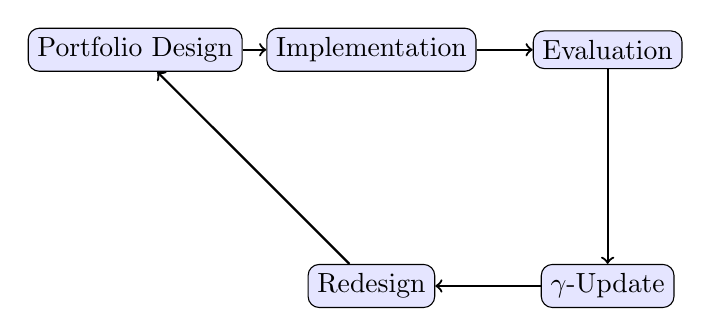
\begin{tikzpicture}[node distance=3cm, auto]
    \node[draw, rounded corners, fill=blue!10] (design) {Portfolio Design};
    \node[draw, rounded corners, fill=blue!10, right of=design] (implement) {Implementation};
    \node[draw, rounded corners, fill=blue!10, right of=implement] (evaluate) {Evaluation};
    \node[draw, rounded corners, fill=blue!10, below of=evaluate] (update) {$\gamma$-Update};
    \node[draw, rounded corners, fill=blue!10, left of=update] (redesign) {Redesign};

    \draw[->, thick] (design) -- (implement);
    \draw[->, thick] (implement) -- (evaluate);
    \draw[->, thick] (evaluate) -- (update);
    \draw[->, thick] (update) -- (redesign);
    \draw[->, thick] (redesign) -- (design);
\end{tikzpicture}
\end{center}

\subsection{Organizational Learning Metriken}

\begin{itemize}
\item \textbf{$\gamma$-Precision:} Reduktion der Konfidenzintervall-Breite über Zeit
\item \textbf{Prediction Accuracy:} $|E_{\text{predicted}} - E_{\text{observed}}|$
\item \textbf{Portfolio Efficiency:} $\frac{E(P)}{Cost(P)}$ über Iterationen
\end{itemize}


%%%%%%%%%%%%%%%%%%%%%%%%%%%%%%%%%%%%%%%%%%%%%%%%%%%%%%%%%%%%%%%%%%%%%%%%%%%%%%%
\section{Worked Examples}
\label{sec:20-examples}
%%%%%%%%%%%%%%%%%%%%%%%%%%%%%%%%%%%%%%%%%%%%%%%%%%%%%%%%%%%%%%%%%%%%%%%%%%%%%%%

\subsection{Beispiel 1: Anna's Kommunales Energie-Portfolio (Vollständig)}

\textbf{Kontext:} Gemeinde mit 10,000 Haushalten, Ziel: -20\% Energieverbrauch, Budget: CHF 200k

\textbf{Schritt 1: Segment-Analyse}
\begin{itemize}[nosep]
\item Present-Biased: 30\%
\item Social-Oriented: 45\%
\item Autonomy-Seeking: 25\%
\end{itemize}

\textbf{Schritt 2: Portfolio-Design}

\begin{table}[htbp]
\centering
\caption{Anna's Energie-Portfolio mit Kohärenz-Check}
\label{tab:20-example-anna}
\renewcommand{\arraystretch}{1.3}
\small
\begin{tabular}{@{}lllcccc@{}}
\toprule
\textbf{Intervention} & \textbf{Typ} & \textbf{Phase} & \textbf{Segment} & \textbf{$E_i$} & \textbf{Kosten} \\
\midrule
$\mathcal{I}_1$: Social Norm Letter & T6 & Awareness & Social & 5\% & CHF 20k \\
$\mathcal{I}_2$: Smart Meter + Feedback & T2+T3 & Action & All & 6\% & CHF 120k \\
$\mathcal{I}_3$: Neighborhood Competition & T6 & Maintenance & Social & 5\% & CHF 40k \\
$\mathcal{I}_4$: Self-Set Goal (Opt-in) & T8 & Trigger & Autonomy & 3\% & CHF 20k \\
\bottomrule
\end{tabular}
\end{table}

\textbf{Schritt 3: Kohärenz-Check}
\begin{itemize}[nosep]
\item C1 (Non-Interference): $\gamma_{12} = +0.5$, $\gamma_{23} = +0.4$, $\gamma_{34} = +0.3$ ✓
\item C2 (Journey-Coverage): Awareness, Trigger, Action, Maintenance ✓
\item C3 (Segment-Coverage): Social + Autonomy + All ✓
\item C4 (Context-Consistency): Alle Haushalt-Kontext ✓
\item \textbf{$C(P) = 1.0$} ✓
\end{itemize}

\textbf{Schritt 4: Effekt-Berechnung}
\begin{align}
E(P) &= (5 + 6 + 5 + 3) + 0.5\sqrt{5 \cdot 6} + 0.4\sqrt{6 \cdot 5} + 0.3\sqrt{5 \cdot 3} + ... \nonumber\\
&= 19\% + 2.7\% + 2.2\% + 1.2\% + 0.8\% = \mathbf{25.9\%}
\label{eq:20-anna-calculation}
\end{align}

\textbf{Ergebnis:} Ziel (-20\%) übertroffen durch Synergie-Effekte.

\subsection{Beispiel 2: Corporate Wellness Portfolio}

\textbf{Kontext:} Unternehmen mit 2,000 Mitarbeitern, Ziel: Gesündere Belegschaft, Budget: CHF 150k

\begin{table}[htbp]
\centering
\caption{Corporate Wellness Portfolio}
\label{tab:20-example-wellness}
\renewcommand{\arraystretch}{1.3}
\small
\begin{tabular}{@{}llll@{}}
\toprule
\textbf{Intervention} & \textbf{Ziel-Segment} & \textbf{Mechanismus} & \textbf{$\gamma$ mit anderen} \\
\midrule
Team Fitness Challenge & Social-Oriented & Peer Pressure + Fun & $+0.5$ mit Feedback \\
Health Dashboard (App) & Present-Biased & Real-time Feedback & $+0.4$ mit Challenge \\
Flexible Wellness Budget & Autonomy-Oriented & Self-Selection & $+0.3$ mit beiden \\
\bottomrule
\end{tabular}
\end{table}

\textbf{Kohärenz-Check:} Keine Crowding-out Risiken (keine T7+T8 Kombination). $C(P) = 0.85$.

\textbf{Erwarteter ROI:} 3.5:1 (basierend auf reduzierter Abwesenheit + Produktivität)

\subsection{Beispiel 3: Nationales Spar-Programm (Multi-Level)}

\textbf{Kontext:} Regierung will nationale Sparquote erhöhen.

\begin{table}[htbp]
\centering
\caption{Multi-Level Spar-Portfolio}
\label{tab:20-example-national}
\renewcommand{\arraystretch}{1.3}
\small
\begin{tabular}{@{}lllc@{}}
\toprule
\textbf{Level} & \textbf{Intervention} & \textbf{Akteur} & \textbf{Zeithorizont} \\
\midrule
L3 (Org) & Auto-Enrollment in Pensionskassen & Arbeitgeber & 1--2 Jahre \\
L4 (Region) & Finanzbildung in Schulen & Kantone & 5--10 Jahre \\
L5 (Nation) & Steuerliche Spar-Anreize & Parlament & 10+ Jahre \\
L5 (Nation) & ``Sparer sind klug''-Kampagne (T5+T6) & Bund & Ongoing \\
\bottomrule
\end{tabular}
\end{table}

\textbf{Cross-Level Kohärenz-Check:}
\begin{itemize}[nosep]
\item L3 Auto-Enrollment + L5 Steuer-Anreize: $\gamma = +0.4$ (verstärken sich)
\item L4 Finanzbildung + L5 Kampagne: $\gamma = +0.5$ (Information + Norm)
\item \textbf{Achtung:} Steuer-Anreize (T7) nicht mit Commitment-Programmen (T8) kombinieren!
\end{itemize}


%%%%%%%%%%%%%%%%%%%%%%%%%%%%%%%%%%%%%%%%%%%%%%%%%%%%%%%%%%%%%%%%%%%%%%%%%%%%%%%
\section{Summary}
\label{sec:20-summary}
%%%%%%%%%%%%%%%%%%%%%%%%%%%%%%%%%%%%%%%%%%%%%%%%%%%%%%%%%%%%%%%%%%%%%%%%%%%%%%%

\begin{tcolorbox}[colback=green!10!white, colframe=green!75!black,
    title=Key Points]

\textbf{Core Message:} Effective behavioral change requires coherent intervention portfolios that leverage complementarities and avoid crowding-out.

\textbf{Key Takeaways:}
\begin{enumerate}
\item \textbf{Portfolio-Formel:} $E(P) = \sum E_i + \sum \gamma_{ij} \sqrt{E_i E_j}$
\item \textbf{Complementarity $\gamma_{ij}$:} Synergy ($>0$) oder Interference ($<0$) zwischen Interventionen
\item \textbf{Vier Kohärenz-Kriterien:} Non-Interference, Journey-Coverage, Segment-Coverage, Context-Consistency
\item \textbf{Crowding-Out vermeiden:} T6+T7 und T7+T8 Kombinationen riskant
\item \textbf{Multi-Level:} Portfolios müssen Cross-Level kohärent sein
\item \textbf{Learning Loop:} Evaluation → $\gamma$-Update → Redesign
\end{enumerate}

\end{tcolorbox}

\begin{tcolorbox}[colback=blue!5!white, colframe=blue!75!black,
    title=Der Vollständige Interventions-Design-Prozess]
\begin{enumerate}[nosep]
\item \textbf{Diagnose:} Journey-Phase + Segment-Identifikation (Kap.\ 18--19)
\item \textbf{Selektion:} Interventions-Typen nach Diagnose (Kap.\ 17)
\item \textbf{Kombination:} Kohärentes Portfolio mit $\gamma_{ij} \geq 0$ (Kap.\ 20)
\item \textbf{Simulation:} Effekte vorhersagen vor Deployment
\item \textbf{Implementation:} Level-spezifische Umsetzung
\item \textbf{Evaluation:} Lernen und Schätzungen aktualisieren
\end{enumerate}
\end{tcolorbox}

%------------------------------------------------------------------------------
\paragraph{Formal Details.}
Die vollständige formale Behandlung findet sich in:
\begin{itemize}[nosep]
\item Appendix HHH (METHOD-TOOLKIT) --- F10 (Complementarity), Axiom HHH-4, Theorem HHH-T7
\item Appendix BB (FORMAL-EQUILIBRIA) --- Portfolio-Equilibria, Tipping-Point-Analysis
\item Appendix R (METHOD-EVAL) --- Evaluations-Protokolle, Attribution-Methoden
\item Appendix FFF (METHOD-REGISTRY) --- $\gamma$-Repository, Organizational Learning
\end{itemize}

%------------------------------------------------------------------------------
\paragraph{What Comes Next.}
\textbf{Kapitel 21} behandelt die \textbf{Limitationen} des Frameworks: Wo funktioniert der Ansatz nicht? Welche Annahmen sind kritisch? Wann versagen Interventionen systematisch?


% -----------------------------------------------------------------------------
% READING PATH BOX
% -----------------------------------------------------------------------------

\begin{tcolorbox}[colback=gray!5!white, colframe=gray!75!black,
    title=Empfohlene Lesepfade]

\textbf{Abgeschlossen:} Der Interventions-Design-Block (Kapitel 17--20)

\textbf{Sie verstehen jetzt:}
\begin{itemize}[nosep]
\item Wie Interventionen systematisch spezifiziert werden (Kap.\ 17)
\item Wie Interventionen auf Journey-Phasen abgestimmt werden (Kap.\ 18)
\item Wie Interventionen auf Segmente ausgerichtet werden (Kap.\ 19)
\item Wie Interventionen zu kohärenten Portfolios kombiniert werden (Kap.\ 20)
\end{itemize}

\textbf{Nächste Schritte:}
\begin{itemize}[nosep]
\item \textbf{Kapitel 21}: Limitations --- Was das Framework nicht kann
\item \textbf{Kapitel 22}: Conclusion --- Zusammenfassung und Ausblick
\end{itemize}

\textbf{Für Implementation:} Appendix HHH (METHOD-TOOLKIT) als operative Referenz
\end{tcolorbox}


% =============================================================================
% POLICY IMPLICATIONS
% =============================================================================

\section*{Policy Implications}

\begin{enumerate}
\item \textbf{Für Gemeinden/Städte:} Portfolio-Ansatz für Energie-, Mobilitäts- und Gesundheitsprogramme. Einzelmaßnahmen verschenken 30--50\% Potential durch fehlende Synergien.

\item \textbf{Für Unternehmen:} HR-Interventionen als kohärentes Portfolio designen. \textbf{Niemals} Commitment-Programme mit finanziellen Anreizen kombinieren (Crowding-out Risiko).

\item \textbf{Für Policy-Maker:} Nationale Reformpakete auf Kohärenz prüfen. Inkonsistente Policies (z.B.\ Norm-Kampagne + Subvention) können sich gegenseitig unterminieren.

\item \textbf{Für internationale Organisationen:} Treaty-Bundles mit positiven Cross-Level Komplementaritäten. Climate + Trade + Development als synergetisches Portfolio, nicht als isolierte Verhandlungen.
\end{enumerate}


% =============================================================================
% END OF CHAPTER 20
% =============================================================================
